\documentclass[9pt,a4paper]{extarticle}
\usepackage[a4paper,top=0.42in,bottom=0.48in,left=0.52in,right=0.52in]{geometry}
\usepackage[T1]{fontenc}
\usepackage{lmodern}
\usepackage{microtype}
\usepackage{booktabs,array,tabularx}
\usepackage{ragged2e}
\usepackage{enumitem}
\usepackage{titlesec}
\usepackage{fancyhdr}
\usepackage{lastpage}
\usepackage{hyperref}
\usepackage{xcolor}
\usepackage{graphicx}
\usepackage{tikz}
\usepackage[most]{tcolorbox}
\usepackage{setspace}
\usepackage{parskip}
\usetikzlibrary{arrows.meta,positioning,calc,fit,shapes.geometric}

% Cline-inspired palette from the reference submission
\definecolor{ink}{HTML}{17191C}
\definecolor{charcoal}{HTML}{34383D}
\definecolor{midgray}{HTML}{666B72}
\definecolor{rulegray}{HTML}{B9BDC2}
\definecolor{softgray}{HTML}{F2F3F4}
\definecolor{papergray}{HTML}{F8F8F8}
\definecolor{white}{HTML}{FFFFFF}

\hypersetup{colorlinks=true,linkcolor=ink,urlcolor=ink,pdftitle={AI Meeting Assistant — Technical Submission},pdfauthor={Jatin Mehra}}
\pagestyle{fancy}\fancyhf{}
\fancyhead[L]{\footnotesize\textsc{AI Meeting Assistant}}
\fancyhead[R]{\footnotesize\textsc{Inter IIT Bootcamp}}
\fancyfoot[C]{\footnotesize\textbf{\thepage\ / \pageref{LastPage}}}
\renewcommand{\headrulewidth}{0.35pt}
\setstretch{0.88}\setlength{\parindent}{0pt}\setlength{\parskip}{2.2pt}
\setlist[itemize]{leftmargin=1.15em,itemsep=0.65pt,topsep=1pt,parsep=0pt}
\renewcommand{\arraystretch}{0.94}

\titleformat{\section}{\large\bfseries\color{ink}}{}{0pt}{}[\vspace{0.15em}\color{rulegray}\titlerule]
\titlespacing*{\section}{0pt}{0.22em}{0.27em}
\titleformat{\subsection}{\normalsize\bfseries\color{charcoal}}{}{0pt}{}
\titlespacing*{\subsection}{0pt}{0.18em}{0.08em}

\newtcolorbox{card}[1][]{enhanced,colback=softgray,colframe=rulegray,boxrule=0.45pt,arc=1.3mm,left=7pt,right=7pt,top=5pt,bottom=5pt,#1}
\newtcolorbox{darkcard}[1][]{enhanced,colback=ink,colframe=ink,coltext=white,boxrule=0pt,arc=1.3mm,left=8pt,right=8pt,top=6pt,bottom=6pt,#1}
\newtcolorbox{notecard}[1][]{enhanced,colback=papergray,colframe=rulegray,borderline west={2pt}{0pt}{charcoal},boxrule=0pt,arc=0pt,left=7pt,right=7pt,top=4pt,bottom=4pt,#1}
\newcommand{\tagline}[1]{{\large\color{charcoal}\itshape #1\par}}
\newcommand{\smallcaps}[1]{\textsc{#1}}
\newcommand{\arrow}{\tikz[baseline=-0.55ex]\draw[-{Latex[length=1.7mm]},line width=.6pt] (0,0)--(.48,0);}
\newcommand{\twocard}[4]{%
\begin{minipage}[t]{0.48\textwidth}\begin{card}\textbf{#1}\par #2\end{card}\end{minipage}\hfill%
\begin{minipage}[t]{0.48\textwidth}\begin{card}\textbf{#3}\par #4\end{card}\end{minipage}}

\begin{document}

% ================================================================
% PAGE 1 — OVERVIEW + ARCHITECTURE
% ================================================================
\thispagestyle{fancy}
{\fontsize{25}{28}\selectfont\bfseries AI Meeting Assistant\par}
\vspace{1pt}
\tagline{From Meeting Audio to Structured, Actionable Records}
\vspace{3pt}
\begin{tabularx}{\textwidth}{@{}X r@{}}
\smallcaps{Inter IIT Bootcamp} & \smallcaps{Multimodel AI Pipeline}
\end{tabularx}
\vspace{3pt}

\begin{minipage}[t]{0.34\textwidth}
\section*{Problem}
Recorded meetings contain decisions, technical terminology, commitments, deadlines and assignments, but raw audio is difficult to review and operationalize.

\section*{Solution}
\begin{card}
\centering
\textbf{AUDIO}\\[-1pt] $\downarrow$\\[-2pt]
\textbf{faster-whisper large-v3 / small + Silero VAD}\\[-1pt] $\downarrow$\\[-2pt]
\textbf{RAW TRANSCRIPT}\\[-1pt] $\downarrow$\\[-2pt]
\textbf{GPT-OSS-20B}\\[-1pt]{\scriptsize Domain Refinement}\\[-2pt]$\downarrow$\\[-2pt]
\textbf{REFINED TRANSCRIPT}\\[-1pt] $\downarrow$\\[-2pt]
\textbf{GPT-OSS-120B}\\[-1pt]{\scriptsize Documentation}\\[-2pt]$\downarrow$\\[-2pt]
\textbf{MEETING RECORD}
\end{card}
\end{minipage}\hfill
\begin{minipage}[t]{0.63\textwidth}
\section*{Three Inspectable Outputs}
\begin{card}
\textbf{Raw Transcript}\quad What the STT model heard; preserved before any LLM transformation.
\vspace{3pt}\hrule\vspace{3pt}
\textbf{Refined Transcript}\quad Domain-aware correction of terminology, names, numbers and grammar while preserving meaning.
\vspace{3pt}\hrule\vspace{3pt}
\textbf{Final Record}\quad Summary, minutes, confirmed decisions, action items, owners, deadlines and evidence.
\end{card}

\vspace{4pt}
\begin{darkcard}
\textbf{Design principle}\par\vspace{2pt}
Each model has one clearly defined responsibility, keeping transcription, refinement and documentation independently inspectable.
\end{darkcard}
\end{minipage}

\vspace{3pt}
\section*{Architecture at a Glance}
\begin{center}
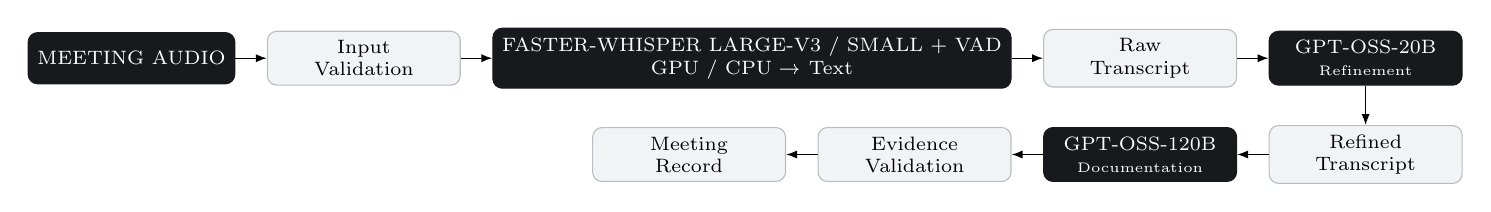
\begin{tikzpicture}[node distance=5mm and 4mm, every node/.style={font=\scriptsize}, box/.style={draw=rulegray,fill=softgray,rounded corners=1.2mm,minimum width=2.45cm,minimum height=0.65cm,align=center}, dark/.style={draw=ink,fill=ink,text=white,rounded corners=1.2mm,minimum width=2.45cm,minimum height=0.65cm,align=center}]
\node[dark] (a) {MEETING AUDIO};
\node[box,right=of a] (b) {Input\\Validation};
\node[dark,right=of b] (c) {FASTER-WHISPER LARGE-V3 / SMALL + VAD\\\scriptsize GPU / CPU → Text};
\node[box,right=of c] (d) {Raw\\Transcript};
\node[dark,right=of d] (e) {GPT-OSS-20B\\\tiny Refinement};
\node[box,below=of e] (f) {Refined\\Transcript};
\node[dark,left=of f] (g) {GPT-OSS-120B\\\tiny Documentation};
\node[box,left=of g] (h) {Evidence\\Validation};
\node[box,left=of h] (i) {Meeting\\Record};
\foreach \x/\y in {a/b,b/c,c/d,d/e,e/f,f/g,g/h,h/i}{\draw[-{Latex[length=1.4mm]},line width=.5pt] (\x)--(\y);}
\end{tikzpicture}
\end{center}

\vspace{3pt}
\twocard{Why preserve raw?}{If the final record is wrong, intermediate representations make it possible to determine whether the issue originated in audio, STT, refinement, documentation or evidence validation.}{System contract}{\small \textbf{Raw} = what was heard\quad \textbf{Refined} = what was improved\quad \textbf{Final} = what is supported.}

\vspace{4pt}
\twocard{Input contract}{Recorded English audio is validated before inference. Empty, corrupt, unreadable or unsupported inputs are rejected explicitly.}{Output contract}{\small Human-readable and machine-readable artifacts are exported without silently replacing earlier valid representations.}

\vspace{4pt}
\begin{darkcard}
\textbf{Core design philosophy}\hfill \smallcaps{Preserve first · Improve second · Extract third}\par
Raw transcript answers \textit{what the speech recognizer heard}; refinement answers \textit{how the conversation can be represented more accurately}; documentation answers \textit{what useful information can safely be extracted}; evidence validation checks the claims before export.
\end{darkcard}

\vspace{4pt}
\begin{tabularx}{\textwidth}{@{}XXX@{}}
\begin{card}\textbf{Inspectable}\par Raw, refined and final representations remain independently visible.
\end{card}&
\begin{card}\textbf{Grounded}\par Decisions and tasks require transcript support.
\end{card}&
\begin{card}\textbf{Actionable}\par The final record is exportable in human and machine-readable forms.
\end{card}
\end{tabularx}

\begin{card}\textbf{Architecture rationale}\quad Preserve the raw conversation, improve it in a dedicated refinement stage, extract structured information separately, then validate claims against evidence. This makes the system inspectable rather than opaque.\end{card}

\vspace{4pt}
\begin{card}
\textbf{Evaluator lens}\quad The architecture makes it possible to inspect three separate questions: What was heard? What was corrected? What was actually supported by the meeting? This separation is the central trust mechanism of the application.
\end{card}

\vspace{4pt}
\begin{notecard}\textbf{KEY TAKEAWAY}\quad The architecture is intentionally a sequence of inspectable semantic transformations rather than one opaque LLM call.
\end{notecard}
\newpage

% ================================================================
% PAGE 2 — STT / WHISPER
% ================================================================
{\fontsize{22}{25}\selectfont\bfseries Stage 1 — Speech Recognition\par}
\tagline{Turning meeting audio into an inspectable timestamped transcript.}
\vspace{4pt}

\begin{minipage}[t]{0.47\textwidth}
\vspace{0pt}
\begin{darkcard}\centering\textbf{faster-whisper large-v3 / small + Silero VAD}\par\vspace{1pt}\scriptsize Audio → Text\end{darkcard}
\begin{card}
\textbf{Input:} recorded English meeting audio\\
\textbf{Output:} timestamped transcript segments\\[2pt]
The STT stage is deliberately isolated from the Groq language-model stages. It creates the first stable textual representation of the conversation.
\end{card}
\end{minipage}\hfill
\begin{minipage}[t]{0.50\textwidth}
\vspace{0pt}
\begin{card}
\textbf{Why local speech recognition?}
\begin{itemize}
\item Local inference keeps the STT layer independent of an external transcription API.
\item No separate hosted STT quota is required during inference.
\item Segment timing remains available to downstream processing and inspection.
\item The same raw artifact can be reused for debugging and evaluation.
\end{itemize}
\end{card}
\end{minipage}

\vspace{4pt}
\begin{card}
\textbf{Hardware-aware defaults}
\quad CUDA available → \texttt{large-v3 + cuda + float16}; CPU fallback → \texttt{small + cpu + int8}. Environment variables \texttt{WHISPER\_MODEL}, \texttt{WHISPER\_DEVICE} and \texttt{WHISPER\_COMPUTE\_TYPE} override these defaults. The transcription call also sets \texttt{condition\_on\_previous\_text=False} to prevent repetitive conditioning loops on long meetings.
\end{card}

\vspace{4pt}
\section*{STT Data Flow}
\vspace{2pt}
\begin{center}
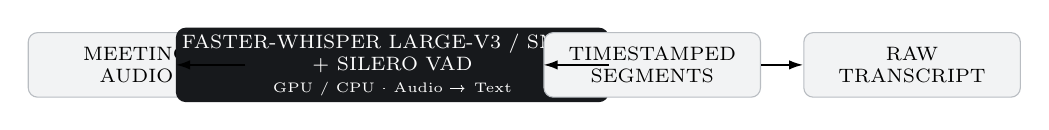
\begin{tikzpicture}[every node/.style={font=\scriptsize}, n/.style={draw=rulegray,fill=softgray,rounded corners=1.2mm,minimum width=2.75cm,minimum height=.82cm,align=center,inner sep=2pt}, dn/.style={draw=ink,fill=ink,text=white,rounded corners=1.2mm,minimum width=2.95cm,minimum height=.82cm,align=center,inner sep=2pt}]
\node[n]  (a) at (0,0)       {MEETING\\AUDIO};
\node[dn] (b) at (3.25,0)  {FASTER-WHISPER LARGE-V3 / SMALL\\+ SILERO VAD\\\tiny GPU / CPU · Audio → Text};
\node[n]  (c) at (6.55,0)  {TIMESTAMPED\\SEGMENTS};
\node[n]  (d) at (9.85,0)  {RAW\\TRANSCRIPT};
\draw[-{Latex[length=1.8mm,width=1.2mm]},line width=.7pt] (a.east)--(b.west);
\draw[-{Latex[length=1.8mm,width=1.2mm]},line width=.7pt] (b.east)--(c.west);
\draw[-{Latex[length=1.8mm,width=1.2mm]},line width=.7pt] (c.east)--(d.west);
\end{tikzpicture}
\end{center}

\begin{notecard}\textbf{Repetition guard}\quad \texttt{condition\_on\_previous\_text=False} prevents conditioning loops and repetitive hallucinations across long meetings while preserving VAD, glossary prompting and segment timestamps.\end{notecard}

\vspace{4pt}
\twocard{What is preserved?}{Segment ordering, transcript text and timing are retained before any refinement. The raw artifact is not silently replaced by later processing.}{Why it matters}{\small A final extraction error can be traced back to the speech-recognition output rather than being hidden inside a single final answer.}

\vspace{4pt}
\section*{Validation Before Inference}
\vspace{2pt}
\begin{tabularx}{\textwidth}{@{}XXX@{}}
\begin{card}\textbf{File validation}\par Empty, corrupt, unreadable or unsupported inputs are rejected explicitly.
\end{card}&
\begin{card}\textbf{Audio readability}\par The pipeline checks that the recording can be processed before invoking downstream models.
\end{card}&
\begin{card}\textbf{Raw artifact}\par A successful STT run produces a stable transcript artifact for later stages.
\end{card}
\end{tabularx}

\vspace{4pt}
\section*{Why the Raw Transcript Is a First-Class Output}
\vspace{2pt}
\begin{card}
The raw transcript is not merely an intermediate variable. It is an explicit product of the system. This creates an auditable boundary between \textbf{what the speech recognizer produced} and \textbf{what later language models changed}. If the refined transcript or final record contains an error, the evaluator can compare representations instead of trusting a single generated result.
\end{card}

\vspace{4pt}
\begin{minipage}[t]{0.48\textwidth}
\begin{darkcard}\textbf{Local STT boundary}\end{darkcard}
\begin{card}
\small
\textbf{Audio} stays in the speech-recognition layer.\par
\textbf{Text} becomes the contract passed to LLM stages.\par
\textbf{Groq} is not responsible for transcription.
\end{card}
\end{minipage}\hfill
\begin{minipage}[t]{0.48\textwidth}
\begin{darkcard}\textbf{Inspectable artifact}\end{darkcard}
\begin{card}
\small
\texttt{raw\_transcript.txt} records the STT result independently from refinement and documentation outputs.
\end{card}
\end{minipage}

\vspace{4pt}
\begin{notecard}\textbf{ENGINEERING NOTE}\quad Preserving the STT artifact prevents downstream LLM fluency from masking speech-recognition errors.
\end{notecard}

\vspace{4pt}
\begin{tabularx}{\textwidth}{@{}XX@{}}
\begin{card}\textbf{Timestamped segments}\par Timing remains available at the STT boundary, making the transcript inspectable beyond plain text.
\end{card}&
\begin{card}\textbf{Downstream contract}\par Later models receive text, not audio, so speech recognition and language reasoning can be evaluated independently.
\end{card}
\end{tabularx}

\vspace{4pt}
\begin{darkcard}
\textbf{Stage contract}\quad \textsc{Audio → timestamped segments → raw transcript. No summarization. No semantic rewriting.}\par
\small The STT stage does not infer decisions, identify owners, correct domain terminology through an LLM, or generate meeting minutes.
\end{darkcard}
\newpage

% ================================================================
% PAGE 3 — REFINEMENT
% ================================================================
{\fontsize{22}{25}\selectfont\bfseries Stage 2 — Domain-Aware Refinement\par}
\tagline{Improve recognition quality without changing what was actually said.}
\vspace{4pt}

\begin{darkcard}
\textbf{openai/gpt-oss-20b}\hfill \textsc{Inference via Groq}\par
\vspace{2pt}
The refinement model receives the raw transcript and performs controlled language cleanup. Its responsibility is to improve transcript quality, terminology and readability while preserving the underlying meaning.
\end{darkcard}

\vspace{4pt}
\section*{What the Refinement Stage Handles}
\begin{tabularx}{\textwidth}{@{}XXXX@{}}
\begin{card}\textbf{Technical terms}\par Domain-specific vocabulary and plausible STT corrections.
\end{card}&
\begin{card}\textbf{Names + acronyms}\par Important entities should not be silently replaced by common alternatives.
\end{card}&
\begin{card}\textbf{Numbers}\par Numerical and monetary values must remain accurate.
\end{card}&
\begin{card}\textbf{Grammar}\par Improve readability and terminology consistency without changing meaning.
\end{card}
\end{tabularx}

\vspace{4pt}
\section*{Protected Semantics}
\begin{center}
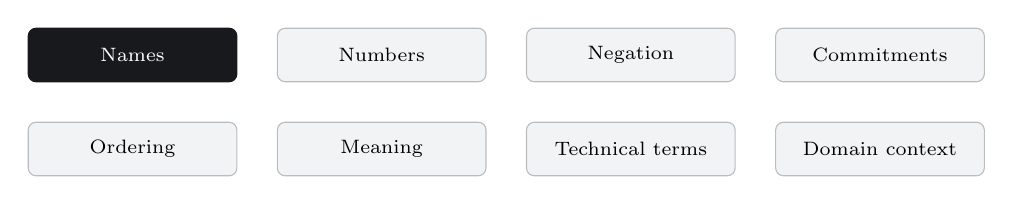
\begin{tikzpicture}[node distance=5mm and 5mm, every node/.style={font=\scriptsize}, n/.style={draw=rulegray,fill=softgray,rounded corners=1mm,minimum width=2.65cm,minimum height=.68cm,align=center}, dn/.style={draw=ink,fill=ink,text=white,rounded corners=1mm,minimum width=2.65cm,minimum height=.68cm,align=center}]
\node[dn] (a) {Names};\node[n,right=of a] (b) {Numbers};\node[n,right=of b] (c) {Negation};\node[n,right=of c] (d) {Commitments};\node[n,below=of a] (e) {Ordering};\node[n,right=of e] (f) {Meaning};\node[n,right=of f] (g) {Technical terms};\node[n,right=of g] (h) {Domain context};
\end{tikzpicture}
\end{center}

\vspace{4pt}
\begin{tabularx}{\textwidth}{@{}XXX@{}}
\begin{card}\textbf{Number safety}\par “2.5 lakh” must not become “25 lakh”. Monetary values are treated as protected information.
\end{card}&
\begin{card}\textbf{Negation safety}\par “We will not deploy this version” must retain its negative commitment.
\end{card}&
\begin{card}\textbf{Commitment safety}\par “We will complete this tomorrow” must preserve its commitment semantics.
\end{card}
\end{tabularx}

\vspace{4pt}
\section*{Optional Glossary Enrichment}
\begin{minipage}[t]{0.48\textwidth}
\begin{card}
\textbf{Glossary can contain}\par
technical terms · product names · project names · domain vocabulary · important names · acronyms
\end{card}
\end{minipage}\hfill
\begin{minipage}[t]{0.48\textwidth}
\begin{card}
\textbf{Failure policy}\par
Glossary extraction is optional. If it fails, the system warns and continues refinement using fallback terminology rather than terminating the mandatory pipeline.
\end{card}
\end{minipage}

\vspace{4pt}
\section*{Long-Meeting Strategy}
\begin{card}
\centering
\textbf{Long transcript} $\rightarrow$ \textbf{Token-aware chunking} $\rightarrow$ \textbf{Sequential GPT-OSS-20B processing} $\rightarrow$ \textbf{Ordered reconstruction} $\rightarrow$ \textbf{Refined transcript}
\end{card}

\vspace{4pt}
\begin{minipage}[t]{0.48\textwidth}
\begin{darkcard}\textbf{Why chunk?}\end{darkcard}
\begin{card}\small Large transcripts can exceed the practical token budget of one structured request. Chunking avoids relying on a fixed meeting-duration assumption.
\end{card}
\end{minipage}\hfill
\begin{minipage}[t]{0.48\textwidth}
\begin{darkcard}\textbf{Why sequential?}\end{darkcard}
\begin{card}\small Chunks are processed in order and reconstructed in their original sequence so the refined transcript remains coherent.
\end{card}
\end{minipage}

\vspace{4pt}
\begin{card}
\textbf{What this stage does NOT do}\par
It does not summarize the meeting, decide what counts as an assignment, invent missing owners, or convert proposals into decisions. Those responsibilities belong to the documentation and evidence stages.
\end{card}

\vspace{4pt}
\section*{Reliability Controls}
\begin{tabularx}{\textwidth}{@{}XX@{}}
\begin{card}\textbf{Structured output}\par Explicit schemas, prompt alignment, validation and retry/backoff protect downstream stages from malformed responses.\end{card}&
\begin{card}\textbf{Audit + fallback}\par Glossary failure is non-fatal; the refined transcript remains a separate artifact for raw-versus-refined inspection.\end{card}
\end{tabularx}

\vspace{4pt}
\begin{darkcard}
\textbf{Stage contract}\quad \textsc{Raw transcript → controlled refinement → refined transcript.}\par
\small Preserve names, numbers, negation, commitments, ordering and meaning; do not summarize or invent.
\end{darkcard}

\vspace{4pt}
\begin{notecard}\textbf{KEY TAKEAWAY}\quad Refinement improves the transcript; it is not permission to rewrite the meeting.\end{notecard}
\newpage

% ================================================================
% PAGE 4 — DOCUMENTATION + EVIDENCE
% ================================================================
{\fontsize{22}{25}\selectfont\bfseries Stage 3 — Documentation + Evidence\par}
\tagline{Turn the refined conversation into a structured record without inventing commitments.}
\vspace{4pt}

\begin{darkcard}
\textbf{openai/gpt-oss-120b}\hfill \textsc{Inference via Groq}\par
\vspace{2pt}
The documentation model receives the refined transcript and asks: \textit{What useful meeting information can safely be extracted from this conversation?}
\end{darkcard}

\vspace{4pt}
\section*{Structured Meeting Record}
\begin{tabularx}{\textwidth}{@{}XXXX@{}}
\begin{card}\textbf{Summary}\par Concise representation of what happened during the meeting.
\end{card}&
\begin{card}\textbf{Decisions}\par Only decisions supported by the conversation.
\end{card}&
\begin{card}\textbf{Action Items}\par Tasks supported by the conversation.
\end{card}&
\begin{card}\textbf{Owners / Deadlines}\par Included only when explicitly stated.
\end{card}
\end{tabularx}

\vspace{4pt}
\section*{Evidence-First Extraction}
\begin{center}
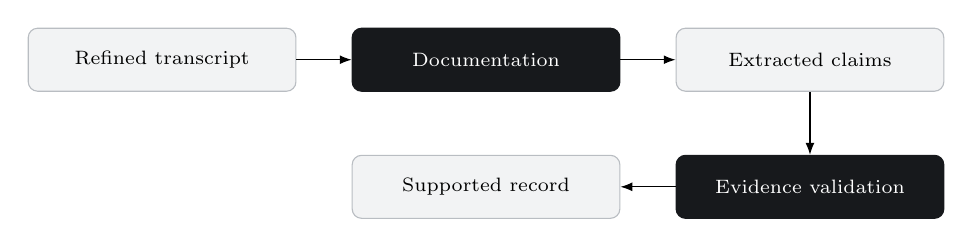
\begin{tikzpicture}[node distance=8mm and 7mm, every node/.style={font=\scriptsize}, n/.style={draw=rulegray,fill=softgray,rounded corners=1.2mm,minimum width=3.4cm,minimum height=.8cm,align=center}, dn/.style={draw=ink,fill=ink,text=white,rounded corners=1.2mm,minimum width=3.4cm,minimum height=.8cm,align=center}]
\node[n] (a) {Refined transcript};
\node[dn,right=of a] (b) {Documentation};
\node[n,right=of b] (c) {Extracted claims};
\node[dn,below=of c] (d) {Evidence validation};
\node[n,left=of d] (e) {Supported record};
\draw[-{Latex[length=1.5mm]}] (a)--(b);\draw[-{Latex[length=1.5mm]}] (b)--(c);\draw[-{Latex[length=1.5mm]}] (c)--(d);\draw[-{Latex[length=1.5mm]}] (d)--(e);
\end{tikzpicture}
\end{center}

\vspace{4pt}
\begin{tabularx}{\textwidth}{@{}XXXX@{}}
\begin{darkcard}\centering\textbf{Proposal}\\$\neq$ Decision\end{darkcard}&
\begin{darkcard}\centering\textbf{Suggestion}\\$\neq$ Assignment\end{darkcard}&
\begin{darkcard}\centering\textbf{Mentioned date}\\$\neq$ Deadline\end{darkcard}&
\begin{darkcard}\centering\textbf{Possibility}\\$\neq$ Commitment\end{darkcard}
\end{tabularx}

\vspace{4pt}
\section*{Examples of Safe Extraction}
\twocard{Discussion}{“We could move this to next week.” is a proposal, not a confirmed decision.}{Assignment}{“Maybe Jatin can handle it.” is a suggestion unless the meeting establishes an actual assignment.}

\vspace{4pt}
\twocard{Missing metadata}{If no owner is stated, owner remains unspecified. If no deadline is stated, deadline remains unspecified.}{Evidence boundary}{A fluent LLM statement is not sufficient evidence. Extracted claims are checked against transcript evidence before entering the final record.}

\vspace{4pt}
\section*{Human + Machine Outputs}
\begin{tabularx}{\textwidth}{@{}XX@{}}
\begin{card}
\textbf{Human-readable}\par
\texttt{minutes.md}\par
\texttt{meeting\_record.md}\par
Summary, decisions, action items and supporting context in an evaluator-friendly format.
\end{card}&
\begin{card}
\textbf{Machine-readable}\par
\texttt{decisions.json}\par
\texttt{action\_items.json}\par
\texttt{meeting\_record.json}\par
\texttt{refinement\_audit.json}
\end{card}
\end{tabularx}

\vspace{4pt}
\begin{card}
\textbf{Why two language models?}\par
GPT-OSS-20B answers: \textit{How can the transcript be represented more accurately without changing its meaning?}\par
GPT-OSS-120B answers: \textit{What decisions and actionable information can safely be extracted?}\par
The separation makes the source conversation and the extracted meeting record independently inspectable.
\end{card}

\section*{Final Record Contract}
\begin{tabularx}{\textwidth}{@{}XXX@{}}
\begin{card}\textbf{Summary}\par What happened, expressed concisely.
\end{card}&
\begin{card}\textbf{Decisions + tasks}\par Only conversation-supported decisions and action items.
\end{card}&
\begin{card}\textbf{Evidence}\par Important extracted claims remain tied to transcript support.
\end{card}
\end{tabularx}

\vspace{4pt}
\begin{card}
\textbf{Output guarantees}\quad The final record distinguishes confirmed information from missing metadata. Unsupported owners, deadlines, decisions or assignments are not filled in merely to make the output look complete.
\end{card}

\vspace{8pt}
\begin{darkcard}
\textbf{Reliability principle}\quad The system prioritizes evidence over fluency. It should fail explicitly rather than silently invent information.
\end{darkcard}
\newpage

% ================================================================
% PAGE 5 — RELIABILITY + ENGINEERING
% ================================================================
{\fontsize{22}{25}\selectfont\bfseries Reliability + Engineering\par}
\tagline{Hardening the pipeline around the failure modes exposed by real testing.}
\vspace{4pt}

\begin{tabularx}{\textwidth}{@{}XX@{}}
\begin{darkcard}\textbf{01 — Long Meeting Token Limits}\end{darkcard}&
\begin{darkcard}\textbf{02 — Structured JSON Reliability}\end{darkcard}
\\
\begin{card}
Long transcripts can exceed the practical generation budget of one request. The final system uses token-aware chunking, sequential processing and ordered reconstruction rather than repeatedly retrying an oversized request.
\end{card}&
\begin{card}
Structured-output validation can fail when generated JSON is malformed. The pipeline uses strict schema alignment, synchronized prompts, sanitization, validation, retry/backoff and JSON-boundary recovery.
\end{card}
\end{tabularx}

\vspace{4pt}
\begin{tabularx}{\textwidth}{@{}XX@{}}
\begin{darkcard}\textbf{03 — Meaning Preservation}\end{darkcard}&
\begin{darkcard}\textbf{04 — Stage Observability}\end{darkcard}
\\
\begin{card}
Regression checks protect negation, monetary values, numerical values, technical terminology, proposal-vs-decision distinctions and unspecified owners/deadlines.
\end{card}&
\begin{card}
The pipeline exposes explicit states: received, validated, transcribing, raw\_ready, refining, refined, documenting, validating, exporting and complete.
\end{card}
\end{tabularx}

\vspace{4pt}
\section*{Retry + Fallback Architecture}
\begin{center}
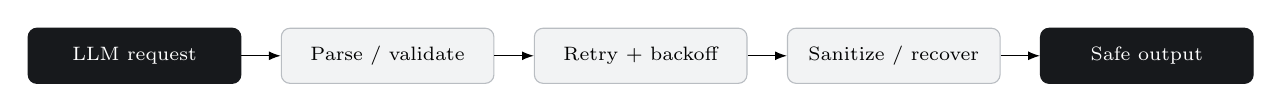
\begin{tikzpicture}[node distance=7mm and 5mm, every node/.style={font=\scriptsize}, n/.style={draw=rulegray,fill=softgray,rounded corners=1.1mm,minimum width=2.7cm,minimum height=.7cm,align=center}, dn/.style={draw=ink,fill=ink,text=white,rounded corners=1.1mm,minimum width=2.7cm,minimum height=.7cm,align=center}]
\node[dn] (a) {LLM request};\node[n,right=of a] (b) {Parse / validate};\node[n,right=of b] (c) {Retry + backoff};\node[n,right=of c] (d) {Sanitize / recover};\node[dn,right=of d] (e) {Safe output};
\draw[-{Latex[length=1.5mm]}] (a)--(b);\draw[-{Latex[length=1.5mm]}] (b)--(c);\draw[-{Latex[length=1.5mm]}] (c)--(d);\draw[-{Latex[length=1.5mm]}] (d)--(e);
\end{tikzpicture}
\end{center}

\vspace{4pt}
\section*{Failure Handling by Criticality}
\begin{center}
\begin{tabularx}{0.94\textwidth}{@{}l X X@{}}
\toprule
\textbf{Component} & \textbf{Failure behavior} & \textbf{Engineering rationale}\\
\midrule
Optional glossary & Warning → continue & Enrichment must never bring down the mandatory pipeline.\\
Refinement & Explicit error → safe stop & Required semantic transformation cannot be silently skipped.\\
Documentation & Explicit error → safe stop & Final structured record must not be fabricated.\\
Evidence validation & Reject unsupported claim & Plausible language is not evidence.\\
\bottomrule
\end{tabularx}
\end{center}

\vspace{4pt}
\twocard{Reasoning-token control}{GPT-OSS models are reasoning models. Long structured requests can consume generation budget before valid JSON appears, so reasoning behavior and output budgets are controlled.}{API-key protection}{\small Exceptions are sanitized before logging so live credentials do not accidentally appear in terminal output or application error messages.}

\vspace{4pt}
\section*{Long-Recording Robustness}
\begin{card}
Long-recording behavior is protected by token-aware chunking, sequential reconstruction and structured-output recovery. Documentation requests use a 2,600-token input budget and 2,048-token output budget, while the STT layer disables previous-text conditioning to reduce repetition loops. The current verification set explicitly exercises these failure modes rather than relying on a single oversized request.
\end{card}

\vspace{4pt}
\section*{Stage-Level Observability}
\begin{card}
\centering\ttfamily\small
received $\rightarrow$ validated $\rightarrow$ transcribing $\rightarrow$ raw\_ready $\rightarrow$ refining $\rightarrow$ refined $\rightarrow$ documenting $\rightarrow$ validating $\rightarrow$ exporting $\rightarrow$ complete
\end{card}

\vspace{4pt}
\begin{tabularx}{\textwidth}{@{}XXX@{}}
\begin{notecard}\textbf{Debuggable}\par A failure can be localized to a stage instead of reported as a generic processing error.
\end{notecard}&
\begin{notecard}\textbf{Resilient}\par Optional enrichment degrades gracefully while required stages fail explicitly.
\end{notecard}&
\begin{notecard}\textbf{Traceable}\par Intermediate artifacts and stage states remain visible for evaluator review.
\end{notecard}
\end{tabularx}

\begin{card}\textbf{Engineering lessons}\quad Observable stages, graceful optional fallbacks, explicit token budgets, structured-output recovery and evidence validation turn real failure modes into testable engineering contracts.\end{card}

\vspace{8pt}
\begin{darkcard}
\textbf{Engineering takeaway}\quad Token limits, malformed structured output, API failures and semantic drift are treated as engineering constraints—not hidden behind a final generated paragraph.
\end{darkcard}
\newpage

% ================================================================
% PAGE 6 — UI + TESTING + STACK + FINAL STATUS\n\small\n\enlargethispage{1.25in}
{\fontsize{21}{23}\selectfont\bfseries UI + Testing + Final Status\par}
\tagline{A compact evaluator surface backed by automated tests and end-to-end verification.}
\vspace{1.5pt}

\begin{minipage}[t]{0.53\textwidth}
\section*{Human-Centered Interface}
\begin{card}
\centering\textbf{Raw Transcript}\hspace{8pt}|\hspace{8pt}\textbf{Refined}\hspace{8pt}|\hspace{8pt}\textbf{Final Output}
\end{card}
\begin{itemize}\setlength{\itemsep}{1pt}\setlength{\parskip}{0pt}
\item \textbf{Raw Transcript} — original timestamped faster-whisper output with Silero VAD and hardware-aware model resolution.
\item \textbf{Refined Transcript} — domain-corrected transcript with preserved meaning.
\item \textbf{Final Output} — summary, minutes, decisions, action items and evidence.
\end{itemize}
\section*{What the Interface Exposes}
\begin{card}
\small
\textbf{Raw view} — unchanged STT artifact and timing.\\
\textbf{Refined view} — corrected terminology without rewriting the conversation.\\
\textbf{Final view} — evidence-grounded decisions and action items.\\
\textbf{Download layer} — intermediate and final artifacts remain independently exportable.
\end{card}
\end{minipage}\hfill
\begin{minipage}[t]{0.44\textwidth}
\begin{darkcard}\centering\fontsize{20}{22}\selectfont\bfseries 105 / 105\par\vspace{1pt}\normalsize automated tests passing\end{darkcard}
\begin{card}\small
\textbf{Coverage}\par\vspace{1pt}
Evidence · Pipeline · Refinement · Safety · UI
\end{card}
\begin{card}\small
\textbf{Real-meeting verification}\par\vspace{1pt}
Current verification covers audio validation, token-aware chunking, refinement, documentation, evidence validation and export through the automated regression suite. Three demo recordings and their output packages are included.
\end{card}
\begin{darkcard}\small
\textbf{Evaluator path}\par\vspace{1pt}
1. Upload a new recording.\\
2. Compare raw vs refined text.\\
3. Inspect evidence-backed decisions.\\
4. Export the complete bundle.
\end{darkcard}
\end{minipage}

\vspace{1.5pt}
\section*{Test Suite}
\scriptsize
\begin{tabularx}{\textwidth}{@{}l X@{}}
\toprule
\textbf{Area} & \textbf{Verified}\\
\midrule
Pipeline & Audio validation, transcription flow, outputs and packaging.\\
Refinement & Chunking, ordering, edit safety, glossary fallback, JSON, retries and sanitization.\\
Safety & Negation, monetary values and safety-sensitive transformations.\\
Evidence & Decision classification, evidence matching and quote extraction.\\
UI & Status streaming, errors and three-stage output layout.\\
\bottomrule
\end{tabularx}

\vspace{1.5pt}
\begin{minipage}[t]{0.46\textwidth}
\section*{Downloadable Output Contract}
\begin{card}\ttfamily\scriptsize
raw\_transcript.txt\\
refined\_transcript.txt\\
minutes.md\\
decisions.json\\
action\_items.json\\
meeting\_record.json\\
meeting\_record.md\\
refinement\_audit.json
\end{card}
\end{minipage}\hfill
\begin{minipage}[t]{0.51\textwidth}
\section*{Technology Stack}
\scriptsize
\begin{tabularx}{\linewidth}{@{}l X@{}}
\toprule
\textbf{Layer} & \textbf{Technology / Role}\\
\midrule
Language & Python — pipeline implementation\\
Speech-to-text & faster-whisper \texttt{large-v3 + float16} GPU / \texttt{small + int8} CPU + Silero VAD — audio → raw transcript\\
Refinement & GPT-OSS-20B — domain-aware correction\\
Documentation & GPT-OSS-120B — structured extraction\\
Inference & Groq — hosted LLM inference\\
UI & Gradio — upload, status, inspection, export\\
Output & JSON / Schema — validated machine-readable record\\
Testing & Pytest — regression suite\\
\bottomrule
\end{tabularx}
\end{minipage}
\vspace{1.5pt}
\section*{PS / Requirement Coverage}
\scriptsize
\begin{center}
{\renewcommand{\arraystretch}{0.72}\begin{tabularx}{0.98\textwidth}{@{}l X l@{}}
\toprule
\textbf{Requirement} & \textbf{Implementation} & \textbf{Status}\\
\midrule
English meeting audio & faster-whisper large-v3 / small + Silero VAD & \textbf{YES}\\
Raw transcript & Dedicated preserved artifact & \textbf{YES}\\
Domain refinement & GPT-OSS-20B & \textbf{YES}\\
Separate documentation stage & GPT-OSS-120B & \textbf{YES}\\
Minutes / summary & Structured meeting record & \textbf{YES}\\
Decisions & Evidence-aware extraction & \textbf{YES}\\
Tasks & Grounded action items & \textbf{YES}\\
Missing owner / deadline & Left unspecified & \textbf{YES}\\
Interactive UI & Gradio & \textbf{YES}\\
Downloads & TXT / MD / JSON & \textbf{YES}\\
New recordings & Dynamic processing pipeline & \textbf{YES}\\
\bottomrule
\end{tabularx}}
\end{center}
\normalsize

\vspace{1.5pt}
\begin{tabularx}{\textwidth}{@{}XX@{}}
\begin{card}[top=3pt,bottom=3pt]\textbf{UI reliability}\par\small Clear stage-level errors, readable transcript text, explicit light-theme styling and separate raw / refined / final views.
\end{card}&
\begin{card}[top=3pt,bottom=3pt]\textbf{Evidence boundary}\par\small Unsupported owners, deadlines or decisions are not invented. Proposal, suggestion and mention remain distinct from commitment.
\end{card}
\end{tabularx}

\vspace{2pt}
\begin{darkcard}
\centering\small
\textbf{Final verification}\quad Upload → Transcribe → Refine → Document → Validate → Export.\\[-1pt]
The system processes recorded English meeting audio through the validated multimodel pipeline and preserves what was said first, then improves and structures it without inventing unsupported meeting facts.
\end{darkcard}

\end{document}
